\documentclass[../main.tex]{subfiles}
\graphicspath{{\subfix{images/}}}

\begin{document}
	\section{Representation of comparator networks}
	A comparator network with n inputs is a sequence of comparators, each comparator is formed by a tuple of channels $C=(i_1,j_1);...;(i_k,j_k)$ where $(1 \leq i_l < j_l \leq n)$. We name size k to the number of comparators the network has. An input $\bar{x}=x_1...x_n \epsilon \{0, 1\}^n$ outputs the network as follows: $\bar{x_0}=\bar{x}$ for $0<l\leq k$, $\bar{x^l}$ is a permutation of $\bar x^{l-1}$ exchanging $\bar x^{l-1}_{i_l}$ and $\bar x^{l-1}_{j_l}$ if $\bar x^{l-1}_{i_l} > \bar x^{l-1}_{j_l}$
	A comparator network is a sorting network if for any n inputs the outputs are the ascending ordered sequence. 
	
	To test that a comparator network is a sorting network we should test all the sequences $2^n$ of \{0, 1\}. This is enough due to the zero-one principle\cite{knuth1997art} that states that a comparator network orders all sequences in \{0,1\} if and only if it sorts all sequences in any ordered set such as the integers set. This way we can test if a comparator network is a sorting network without having to test the n! combinations of sequences.
	
	\begin{figure}[H]
		\centering
		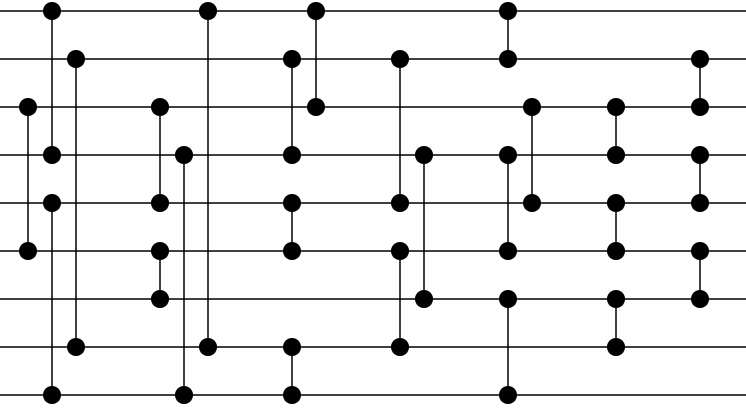
\includegraphics[scale=0.8]{images/Size8SortingNetwork}
		\caption{Size 8 sorting network}
		\label{fig:images/Size8SortingNetwork}
	\end{figure}
\end{document}